\section{Schätztheorie}

\subsection{Bayes-Filterung}
Der allgemeinste Algorithmus zur Berechnung von Posterioren Wahrscheinlichkeiten, in unserem Projekt für die Position und Ausrichtung des Laufroboters, ist durch den Bayes-Filter gegeben.
 Dieser Algorithmus berechnet die Wahrscheinlichkeitsverteilung aus der Messung und Befehlen. Wir werden zuerst den grundlegenden Algorithmus mit den bisherigen Annahmen angeben. Eine Ablauf des Bayesfilterung-Algorithmus ist in der folgenden Abbildung dargestellt.

{\centering
 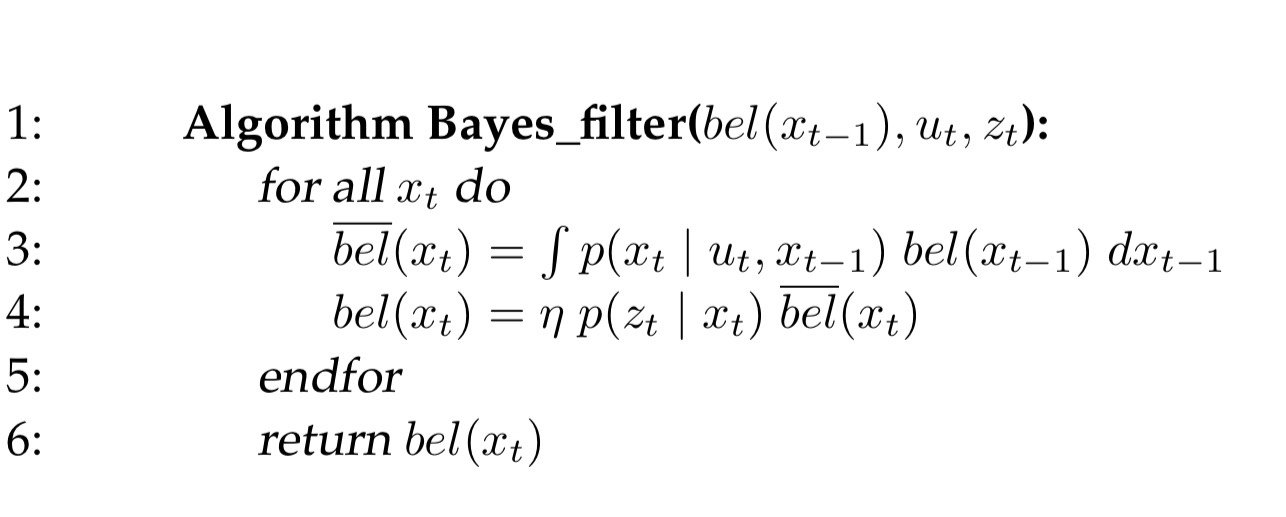
\includegraphics[width=12cm]{Images/image_6483441.jpg}}

Die gewünschte Ausgabe ist eine Schätzung des Zustands $bel(x_{t})$ zur Zeit $t$ (In unsere Projekt ist dies die Wahrscheinlichkeitsverteilung des aktuellen Zustands). Die Eingabe besteht aus der Schätzung des Vorgängerzustands $bel(x_{t-1})$, zusammen mit der letzten Befehl $u_{t}$ und der letzten Messung $z_{t}$. Die gesuchten Werte sind die Posterioren Wahrscheinlichkeiten $bel(x_{t})$ zum Zeitpunkt $t$. Dieser Updateschritt wird rekursiv angewendet. Erst wird das Schätzung $bel(x_{t})$ aus der Schätzung $bel(x_{t-1})$ zuvor berechnet. Deshalb besitzt die Bayes-Filter-Algorithmus aus zwei wesentlichen Schritten: Prediction und Update. Veranschaulicht in folgendem Diagramm.

{\centering
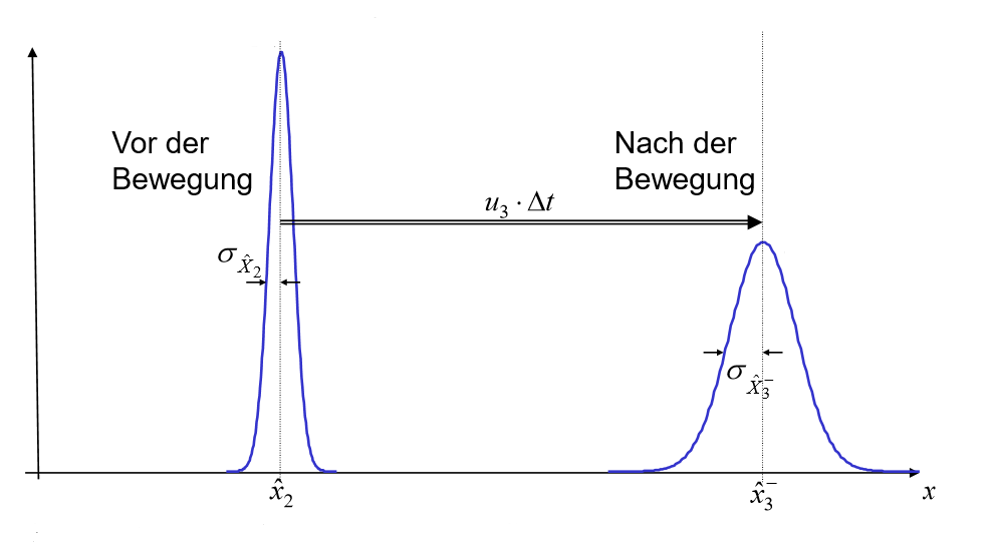
\includegraphics[width=8.2cm]{Images/prediction.png}}
{\centering
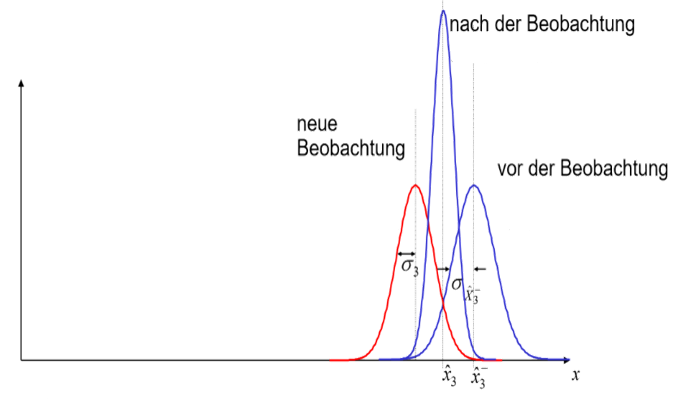
\includegraphics[width=8.2cm]{Images/update.png}}


\clearpage
\subsection{Kalman-filter}

Der Kalman-Filter dient dazu, Fehler in realen Messwerten zu reduzieren und Schätzungen für nicht messbare Systemgrößen zu liefern. Voraussetzung dabei ist, dass die interessierenden Werte durch ein mathematisches Modell beispielsweise in Form von Bewegungsgleichungen beschrieben werden können. Der Filter ermöglicht den Einsatz in Echtzeitsystemen verschiedener technischer Bereiche. Dazu zählen u.a. die Auswertung von Radarsignalen oder GPS-Daten zur Positionsbestimmung sich bewegender Objekte (Tracking). Deshalb ist er für unsere Projekt zur Positionschätzung geeignet. 
 
Das Kalman-Filter bestimmt wie das Bayes Filter seine Schätzungen rekursiv. Während das Bayes-Filter jedoch mit der Schätzfunktion jeweils die exakte Verteilung des aktuellen Zustands bestimmt, werden beim Kalman-Filter in jedem Schritt nur der Erwartungswert des Zustands und die Kovarianz dieser Schätzung bestimmt. Zur Initialisierung der Rekursion wird für $k = 0$ die Anfangsschätzung $\widehat{X}_{0}=X_0 $ mit der Kovarianz $P_{0}$ gewählt.Da der Kalman-Filter den Zustand eines Systems aus dem Eingangs- und Ausgangssignal schätzt, wird es als Zustandsschätzer bezeichnet. Das Kalman-Filter bestimmt zu jedem Zeitpunkt den Erwartungswert und die Kovarianz der zu schätzenden Größe. Die Berechnungsvorschrift wird nachfolgend hergeleitet.

\subsubsection{Prädiktionsschritt }
Im Prädiktionsschritt soll die beste Schätzung von $X_{k}$ und die zugehörigen Kovarianz aus der Befehlsfolge mit den zugehörigen Messungen $u_{1},...,u_{k},y_{1},...,y_{k-1} $ und $X_{0},P_{0}$ bestimmt werden. Außerdem ist die Schätzung des vorherigen Zeitschritts $\widehat{x}_{k-1}$ und deren Kovarianz $P_{k-1}$ verfügbar, welche die beste erwartungstreue Schätzung von $X_{k-1}$ unter Nutzung aller oben genannter Information außer $u_{k}$ darstellt.

Der Erwartungswert des Systemzustands wird mit Hilfe der Systemgleichung bestimmt wobei der unbekannte Zustand $X_{k-1}$ durch die aktuelle Schätzung $\widehat{x}_{k-1}$ ersetzt werden kann.

\begin{equation}
\tag{3.1}
\widehat{x}_{k}^{-}=E{X_{k}}=E{AX_{k-1}+Bu_{k}+R_{k}}
\end{equation}

Die Kovarianz der Prädiktion lautet damit
\begin{equation}
\tag{3.2}
{P}_{k}^{-}=Cov({X}_{k}^{-})=AP_{k-1}A^{T}+\Sigma_{R}
\end{equation}

In der Umformung wurde genutzt, dass das Systemrauschen zum Zeitpunkt $k$ unkorreliert mit
Größen vorheriger Zeitpunkte ist. Der erste Summand der Kovarianz gibt die in Schritt $k-1$ bestehende
Unsicherheit gewichtet mit der Systemdynamik A wieder. Durch den zweiten Summanden
kommt noch das neue Systemrauschen $R_{k}$ hinzu. Gleichungen $(3.1)$ und $(3.2)$ bestimmen somit, wie aus der Schätzung des Systemzustands und deren Kovarianz zum vorherigen Zeitpunkt$ k-1$ eine Prädiktion derselben Größen für den Zeitpunkt k.

\subsubsection{Innovationsschritt}
Im Innovationsschritt soll zusätzlich die aktuelle Beobachtung $y_{k}$ berücksichtigt werden. In dieser Schritt wird erst die Verstärkungsmatrix (Kalman Gain) berechnet:

\begin{equation}
\tag{3.3}
K=\widehat{P}_{k}^{-}C^{T}(CP_{k}^{-}C^{T}+\Sigma_{S})^{-1}
\end{equation}
Entsprechend erfolgt die Innovation linear, als gewichtete
Summe der aktuellen Schätzung und einer Innovation, die proportional zum aktuellen Beobachtungsresiduum ist
\begin{equation}
\tag{3.4}
\widehat{x}_{k}=\widehat{x}_{k}^{-}+K(y_{k}-C\widehat{x}_{k}^{-})
\end{equation}
Unter Nutzung der Voraussetzung, dass das Beobachtungsrauschen $S_{k}$ unkorreliert ist mit der Prädiktion, lässt sich die Kovarianz der Innovation berechnen gemäß

\begin{equation}
\tag{3.5}
P_{k}=(I-KC)P_{k}^{-}(I-KC)^{T}+K\Sigma_{S}K^{T}
\end{equation}
Wie noch gezeigt wird, lässt sich dieser Ausdruck für die optimale Verstärkungsmatrix des KalmanFilters K weiter vereinfachen zu

\begin{equation}
\tag{3.6}
P_{k}=(I-KC)P^{-}_{k}
\end{equation}


\subsection{Partikel-Filter}
Als Vergleichsverfahren für den SE(2)-Filter wird der Partikel-Filter verwendet. Partikel-Filter ist auch als SMC-Methode bekannt. Die Funktionsweise der Filterung ebenfalls auf der Bayes-Filterung. Der Partikelfilter ist eine alternative nichtparametrische Implementierung des Bayes-Filter. Partikelfilter nähern sich der posterioren Wahrscheinlichkeit an. 
Es wird eine große Anzahl an Partikeln mit verschiedenen Parametern zu generiert und in dem den Zustandsraum zu füllen ist die Schlüsselidee.
Die Posteriori Schätzung $bel(x_{t})$ soll durch eine Zufallsmenge dargestellt werden. Von dieser posterioren Verteilung werden Zustandsproben gezogen. Anstatt die Verteilung durch eine parametrische Form darzustellen, stellt der Partikelfilter die Verteilung durch eine Menge von Stichproben aus der aktuelle Verteilung dar. Die ganze Prozess kann durch folgendes Diagramm veranschaulicht werden.

    {\centering
    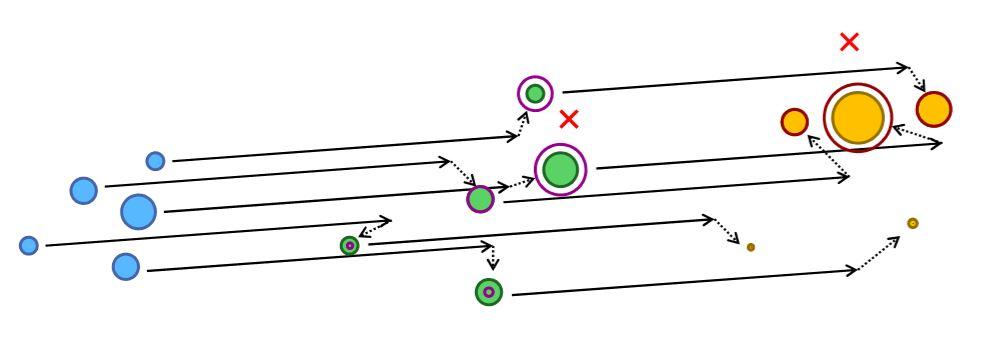
\includegraphics[width=15cm]{Images/pf.jpg}}
    
Das oben gezeigtem Bild beschreibt den Prediction- und Update-Schritt des Partikelfilters. Die blauen Partikel ist die Stichproben des aktuellem Zustands, durch die Zustandsüberführung werden die Partikel für den nächsten Schritt erzeugt (in Bild sind dies die grünen Partikel), im nächsten Schritt werden die Partikel durch die aktuelle Messungen korrigiert. Daraus bekommen wir posteriore Stichproben.
In unsere Projekt wird die Partikel-Filter durch die PF-Klasse von robotics system toolbox eingesetzt. Damit können wir direkt das Systemmodell für die Zustandüberführung und das Messmodell des Partikel-Filter anpassen.